% !TEX root = ./repair.tex

\section{Simulation studies}
\label{sec:experiments}
%\let\beta\theta

In this section we discuss experimental results for over-paramaterized linear models, random feature models, and neural networks, illustrating and confirming the theoretical results presented in the previous sections.
In all of our experiments, the \texttt{quantreg} package in $R$ is used to carry out the median regression (quantile regression for quantile level $\tau = \frac{1}{2}$) of \eqref{eq:keylp} using the Frisch-Newton interior point algorithm to solve the linear program (method \texttt{fn} in this package).


\subsection{Over-parameterized linear models}


We begin by giving further details of the simulation briefly discussed
in Section~\ref{sec:overview}. In this experiment we simulate underdetermined linear models where $p > n$.
We generate $n$ data points $(X_i, y_i)$ where
$y_i = X_i^T \theta^* + w_i$ with $w_i$ an additive noise term. We then compute the minimum norm estimator
\begin{equation}
  \hat\theta = X^T (X X^T)^{-1} y
\end{equation}
The estimated model is corrupted to
\begin{equation}
  \eta = \hat\theta + z
\end{equation}
where $z_j \sim (1-\epsilon) \delta_0 +\epsilon Q$. The corrupted estimator is then repaired by performing median regression:
\begin{align}
  \tilde u &= \argmin \|\eta - X^T u\|_1 \\
  \tilde \theta &= X^T \tilde u.
\end{align}

The design is sampled as $X_{ij} \sim N(0,1)$ and we take $\theta_j^* \sim N(0,1)$ and $Q = N(1,1)$. In the plots shown
in Figure~\ref{fig:exp1} the sample size is fixed at $n=100$ and the dimension $p$ is varied according to $p/n=200/j^2$
for a range of values of $j$. The plots show the empirical probability of exact repair $\tilde\theta = \hat\theta$ as a function of $\epsilon$. Each point on the curves is the average repair success over $500$ random trials.
The roughly equal spacing of the curves agrees with the theory, which indicates that $\sqrt{n/p}/(1-\epsilon)$ should be sufficiently small for successful repair. The right plot in Figure~\ref{fig:exp1b} shows the per-coefficient repair probability, where the left plot shows the probability that the entire model is repaired; in this plot the sample size is $n=50$.

\begin{figure}[ht]
  \begin{center}
    \begin{tabular}{cc}
      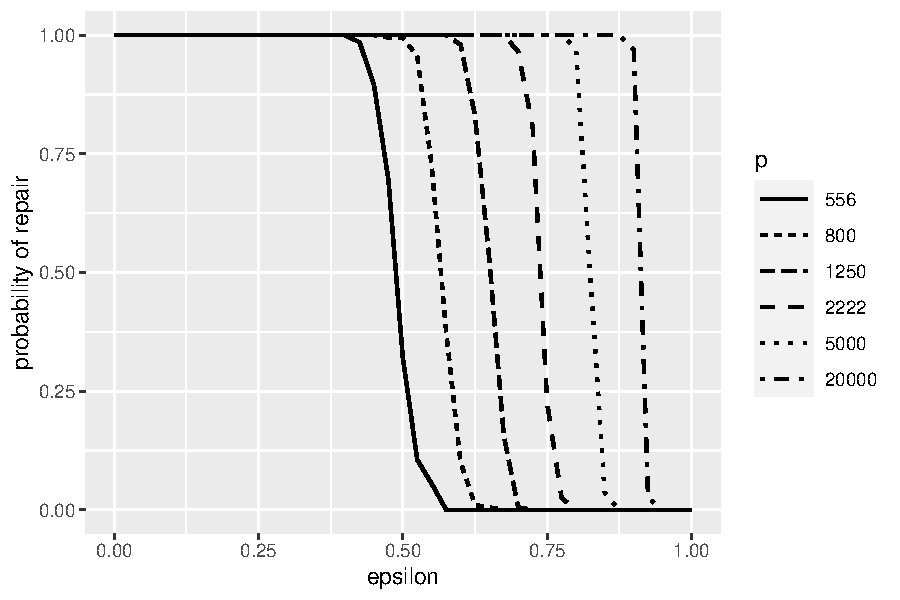
\includegraphics[width=.47\textwidth]{fig/plot-linear-100} &
      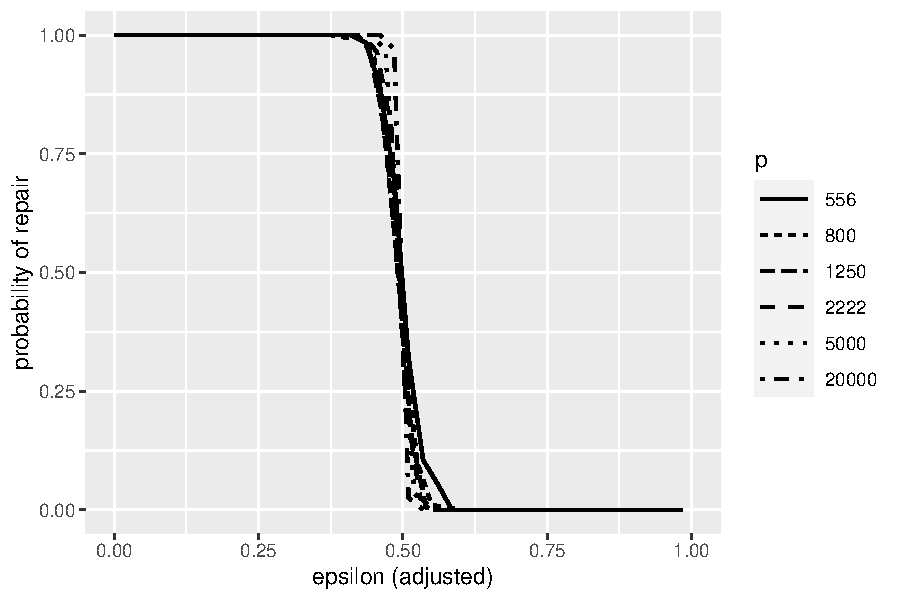
\includegraphics[width=.47\textwidth]{fig/plot-linear-100-adj}\\[-10pt]
    \end{tabular}
    \caption{Model repair for underdetermined linear models $y=X^T\theta + w$ with $p>n$. The left plot shows the empirical probability of successful model repair for $n=100$ with the model dimension $p$
    varying as $p/n = 200 /j^2$, for $j=1,\ldots, 7$. Each point is an average over 500 random trials. The covariates are sampled as $N(0,1)$ and the corruption distribution is $Q=N(1,1)$. The right plot shows the repair probablity as a function
    of the adjusted corruption probability $\tilde\epsilon_j = \epsilon + c'\cdot j - \frac{1}{2}$ for $c'=0.085$.}
    \label{fig:exp1}
    \vskip10pt
    \begin{tabular}{cc}
      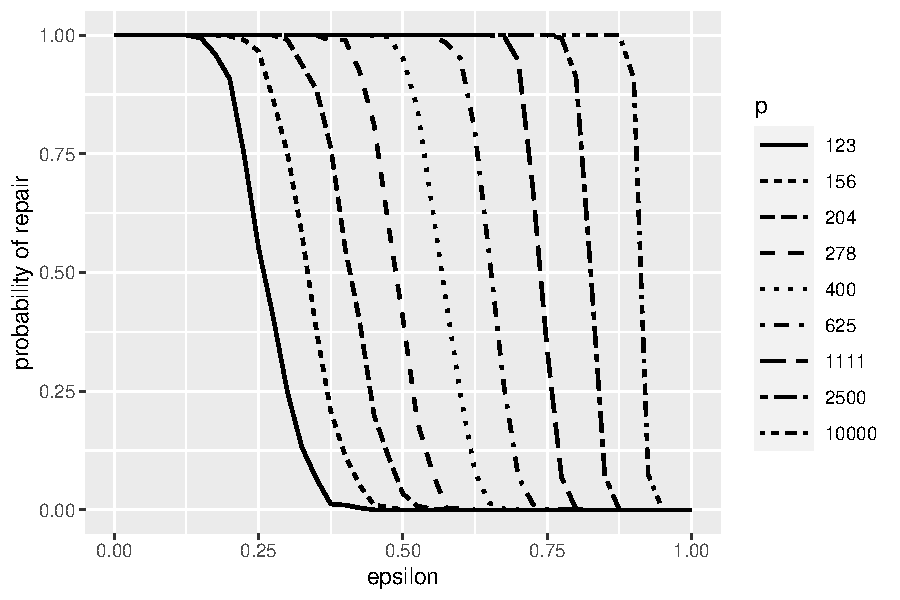
\includegraphics[width=.47\textwidth]{fig/plot-linear-total-50} &
      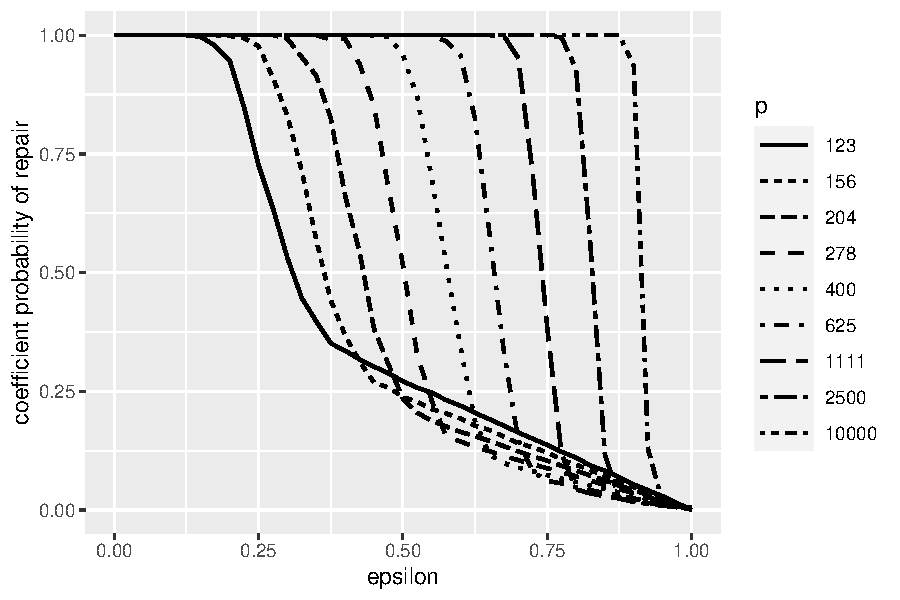
\includegraphics[width=.47\textwidth]{fig/plot-linear-sum-50}\\[-10pt]
    \end{tabular}
  \end{center}
\caption{Left: Empirical probability of successful model repair for $n=50$ with the model dimension $p$
varying as $p/n = 200 /j^2$. Right: Per-coefficient probability of successful repair.}
\label{fig:exp1b}
\end{figure}


\begin{figure}[ht]
  \begin{center}
    \begin{tabular}{c}
      $n=50$ and $p=500$ fixed, varying mean $\mu$\\
      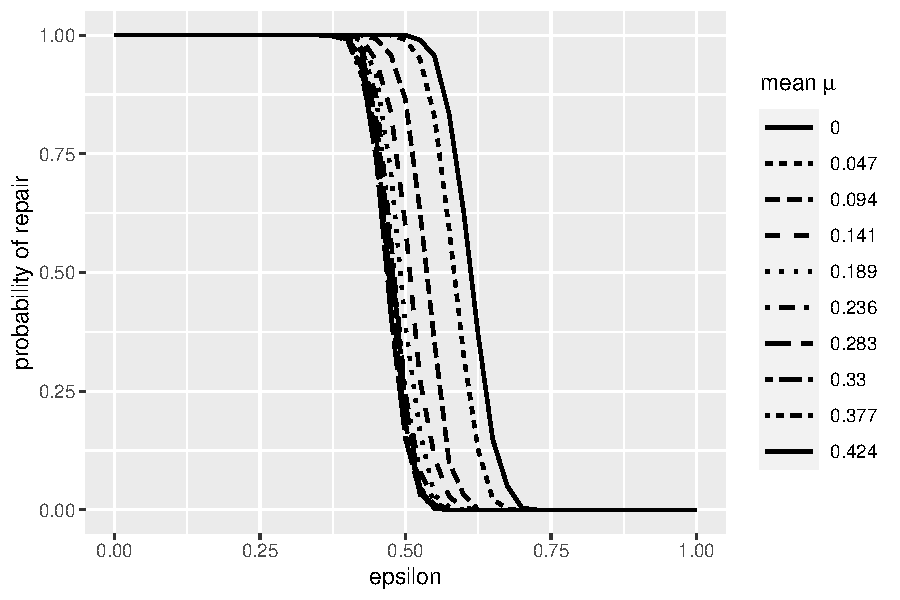
\includegraphics[width=.55\textwidth]{fig/plot-linear-mean-shift-50}
    \end{tabular}
  \end{center}
\caption{Model repair for linear models with design entries $X_{i,j}\sim N(\mu, 1)$,
where the mean $\mu$ is varied and the sample size and dimension are fixed at $n=50$ and $p=500$. Consistent with Theorem~\ref{thm:main-improved}, a smaller corruption fraction $\epsilon$ is tolerated as the mean $\mu$ increases. In the plot above, the means are chosen as $\mu_j = c_j/\sqrt{n}$ for $c_j$ varying between zero and two.}
\label{fig:mean}
\end{figure}

\subsection{Varying the mean}


In this experiment we simulate over-parameterized linear models
with nonzero mean. The data are generated as $X_{ij} \sim N(\mu,1)$
independently, where we vary the mean $\mu$ and fix the dimension $p=500$ and sample size $n=50$.
The probability of successful repair is shown in Figure~\ref{fig:mean}.


As expected, the fraction $\epsilon$ that allows successful repair decreases; it appears to saturate at some fixed value $\epsilon_{\min}$. The mean $\mu$ cannot be made too large because it causes the design $X$ to become ill-conditioned, and the median regression fails.

The inequality in Condition $A$ in this case takes the form
\begin{align*}
  \left\|\frac{1}{m}\sum_{i=1}^m c_i a_i\right\|^2 &\leq \frac{(1+\mu^2)k}{m} + \mu^2 k
   \equiv \frac{(1+\mu^2)n}{p} + \mu^2 n.
   %  = \frac{(1+\mu^2)n}{p} + c_j.
\end{align*}
The means $\mu$ in Figure~\ref{fig:mean} are taken to be $\mu_j = c_j / \sqrt{n}$ as $c_j$ varies between zero and two.

\subsection{Random features models trained with gradient descent}

In this experiment we simulate over-parameterized random features models.
We generate $n$ data points $(X_i, y_i)$ where
$y_i = X_i^T \theta^* + w_i$ with $w_i$ an additive noise term. The covariates are generated
as a layer of a random neural network, with $X_i = \tanh(WZ_i)$ where $Z_i \in\reals^d$ with $Z_{ij} \sim N(0,1)$
and $W\in\reals^{p\times d}$ with $W_{ij} \sim N(0, 1/d)$. We then approximate the least squares
solution using gradient descent intialized at zero, with updates
\begin{equation}
  \hat\theta^{(t)} = \hat\theta^{(t-1)} + \frac{\eta}{n} X^T R^{(t-1)}
\end{equation}
where the residual vector $R^{(t-1)}\in\reals^n$ is given by $R_i = (y_i - X_i^ T\hat\theta^{(t-1)})$.
The step size $\eta$ is selected empirically to insure convergence in under $1{,}000$ iterations.
Figure~\ref{fig:rf} shows two sets of results, for $n=50$ and $n=100$. For each value of the final dimension $p$,
three values of the original data dimension $d$ are selected: $d=p$, $d=\lceil 2p/3\rceil$,
and $d=\lceil p/2\rceil$. The recovery success curves for gradient descent are similar to those obtained for the minimal norm solution. The results are also similar if the ReLU activation function is used, as long as the population mean of the features is subtracted.

\begin{figure}[ht]
  \begin{center}
    \begin{tabular}{cc}
      {\scriptsize $n=50$} & {\scriptsize $n=100$} \\
      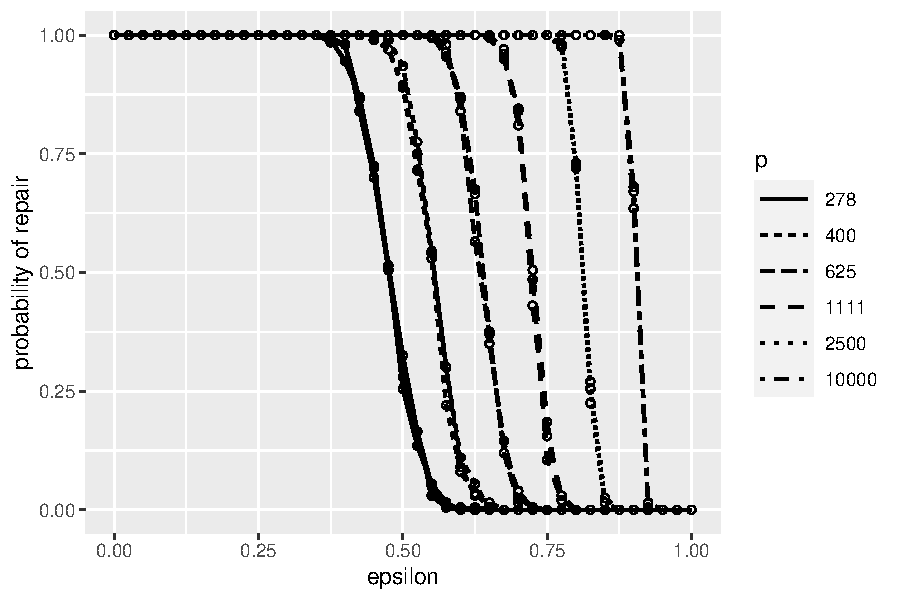
\includegraphics[width=.47\textwidth]{fig/plot-rf-50} &
      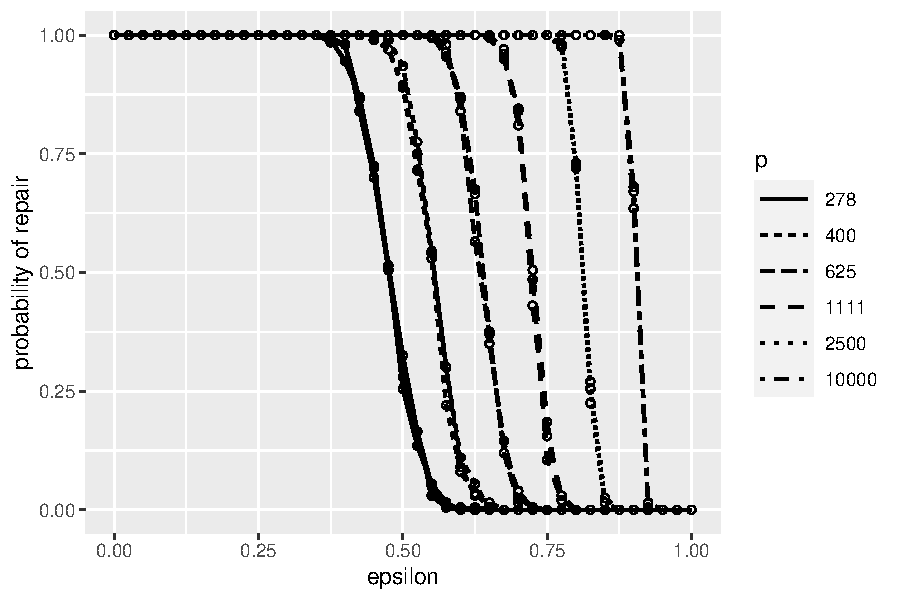
\includegraphics[width=.47\textwidth]{fig/plot-rf-100}\\[-10pt]
    \end{tabular}
  \end{center}
\caption{Model repair for random feature models $y=\psi(XW)\theta + w$ with $p>n$, where $\psi(\cdot) = \tanh(\cdot)$
for $n=50$ (left) and $n=100$ (right). For each value of $p$, three values of $d$ are evaluated, $d=p$, $d=\lceil 2p/3\rceil$,
and $d=\lceil p/2\rceil$; the results are effectively the same for each $d$. The curves are very similar when $\tanh$ is replaced by ReLU, as long as the population mean is subtracted from the features.}
\label{fig:rf}
\end{figure}

\subsection{Neural networks}
\vskip10pt

In this set of simulations we investigate repair algorithms for neural networks. We report results using a single layer and the use of the hyperbolic tangent activation function. Results using the ReLU activation are similar as long as the features are centered.

As described in Section~\ref{sec:neural}, we consider two possible ways of training the models---with our without a forward pass to train the network parameters in stages. In the first approach, the network is trained using gradient descent, and the weights $\hat W\in\reals^{d\times p}$ are then fixed. Next, the weights $\beta\in\reals^p$ are initialized at zero, and gradient descent over $\beta$ is carried out using features
$\tilde X = \psi(X\hat W)$. This two-pass approach allows for exact repair, and only the initial weights $W(0)$ need to be accessed by the repair algorithm, using the seed value used in the pseudorandom number generator.

The left plot in Figure~\ref{fig:ann} shows the behavior of the linear program for exact repair when using this two-stage training algorithm.
The sample size is fixed at $n=50$, the number of ``neurons'' $W_j$ varies as $p$, and we take $d=p/2$. It can been seen that similar repair curves are obtained as for linear models, but the curves are shifted toward the left, indicating an overall smaller probability of successful repair. This makes sense intuitively since for successful repair it is required that
$O(p^2)$ parameters are recovered---each of the $p$ columns $W_j\in\reals^d$ in addition to the vector $\beta\in\reals^p$.

In the second approach, the neural network is trained using standard gradient descent, without a final forward pass. As described in
Section~\ref{sec:neural}, when trained in this manner the column space of $\tilde X = \psi(X W)$ is continually changing. However,
the ``neural tangent kernel'' analysis ensures that the linear program will approximately recover the trained parameters after they are corrupted by additive noise. This is seen in the center and right plots of Figure~\ref{fig:ann}, which show the
average squared errors $(\tilde W_{ij} - \hat W_{ij})^2$ and $(\tilde \beta_j - \hat\beta_j)^2$. All of these results are consistent with our analysis, and suggest that the growth conditions on $d$ and $p$ in the results of our theorems are conservative.

\begin{figure}[t]
  \begin{center}
    \vskip15pt
    \begin{tabular}{ccc}
    \hskip-6pt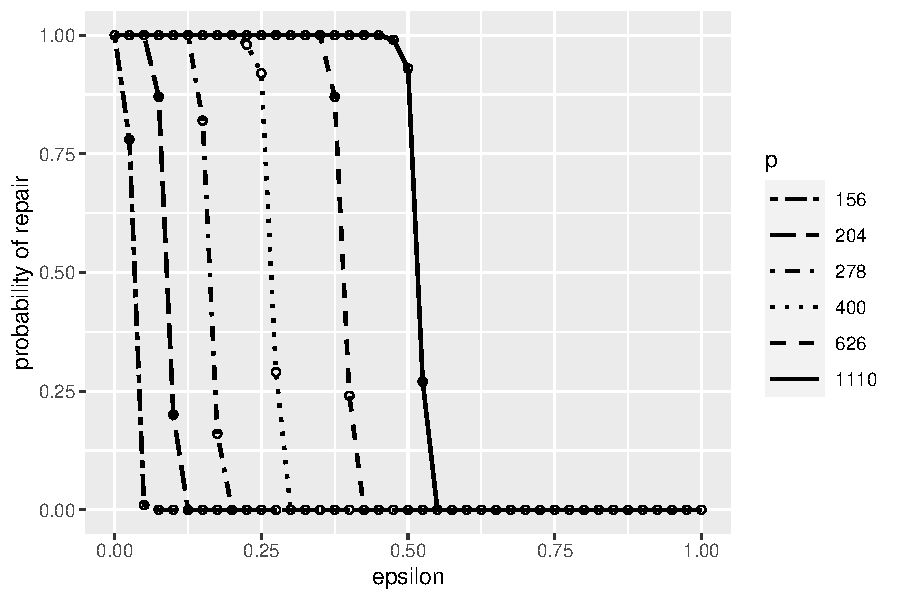
\includegraphics[width=.32\textwidth]{fig/ann-tanh-retrain-n=50-trials=100} &
    \hskip-6pt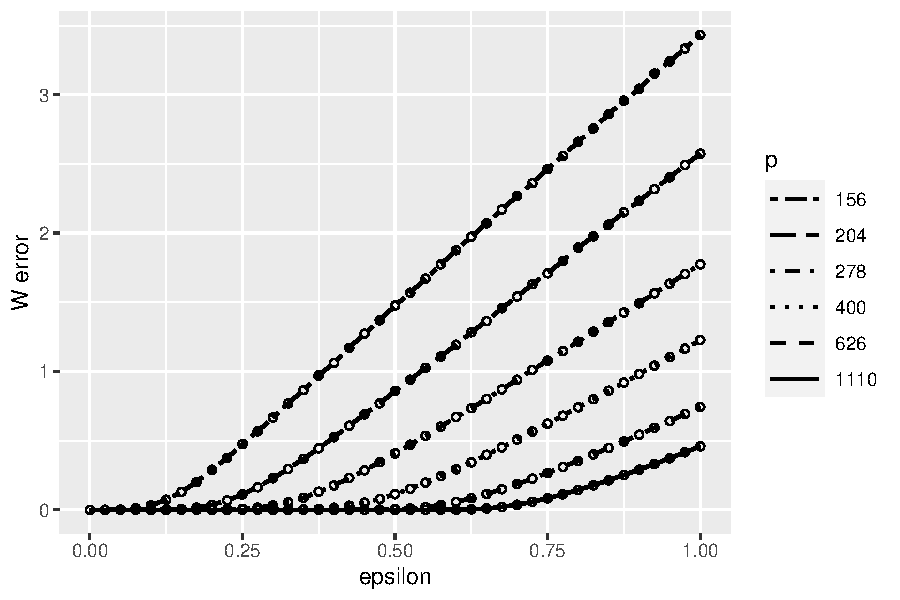
\includegraphics[width=.32\textwidth]{fig/ann-tanh-retrain=F-n=50-trials=100-W_error} &
    \hskip-6pt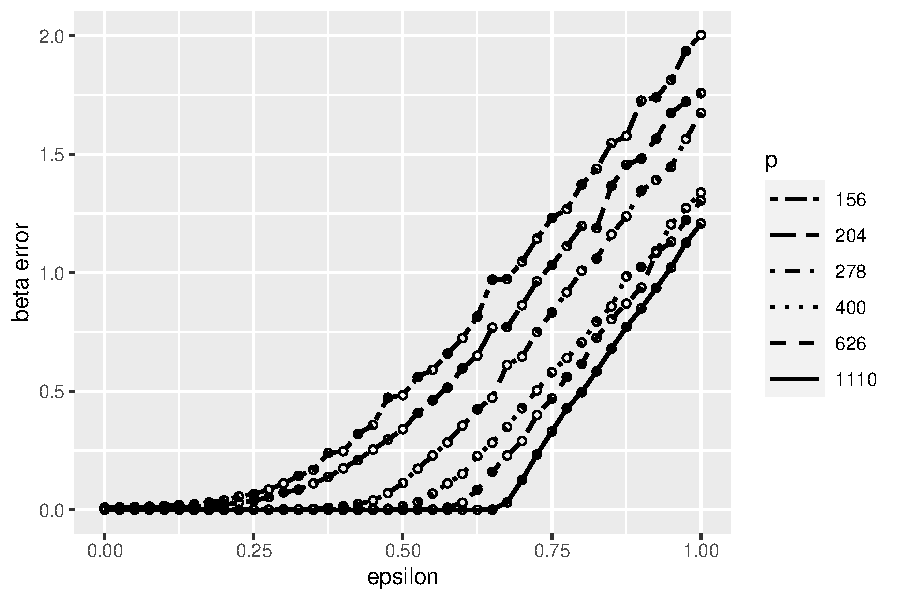
\includegraphics[width=.32\textwidth]{fig/ann-tanh-retrain=F-n=50-trials=100-beta_error}

    \end{tabular}
  \end{center}
\caption{Model repair for neural networks with a single hidden layer. The sample size is fixed at $n=50$, the number of hidden units is $p$, and the input dimension is $d=p/2$; the dimenson of the design is $X\in\reals^{n\times d}$, and the hidden layer is generated
as $\tanh(XW)$ where $W\in\reals^{d\times p}$. The predicted values are $\hat y = \tanh(XW)\beta$.
Left: The neural network is trained with gradient descent after initializing $W_{ij}$ as $N(0, 1/d)$
and $\beta \sim N(0, I_p)$. After training, a forward pass is made where $\hat W$ is fixed and the parameters
$\beta$ are retrained using gradient descent initialized at zero. This enables exact repair by running the linear program in stages, first repairing $\hat W$, and then repairing $\hat \beta$. In order to obtain a successful repair, it is required that all of the columns of $\hat W$ and the vector $\hat\beta$ are exactly recovered, up to numerical precision. Center and right: The neural network is trained with gradient descent using random initialization of $W$ and $\beta$; no forward pass is made after training. The weight matrix $W$ and weight vector $\beta$ are then not repaired exactly. The center and right plots show the average $L_2$ error in the estimated coefficients $W_{ij}$ and $\beta_j$ as a function of the corruption fraction $\epsilon$. In all plots, each point is the average over $100$ random trials. }
\label{fig:ann}
\end{figure}
